\documentclass[letterpaper]{article}
% Set target color model to RGB
\usepackage[inner=1.5cm,outer=1.5cm,top=1.5cm,bottom=1.5cm]{geometry}
\usepackage{setspace}
\usepackage[rgb]{xcolor}
\usepackage{lmodern}
\usepackage{float}
\usepackage{verbatim}
\usepackage{subcaption}
\usepackage{amsgen,amsmath,amstext,amsbsy,amsopn,tikz,amssymb,tkz-linknodes}
\usepackage{fancyhdr}
\usepackage[colorlinks=true, urlcolor=blue,  linkcolor=blue, citecolor=blue]{hyperref}
\usepackage[colorinlistoftodos]{todonotes}
\usepackage{rotating}
\usepackage{listings}
\usepackage{minted}
\usemintedstyle{vs}
%\usetikzlibrary{through,backgrounds}
\hypersetup{%
pdfauthor={Ashudeep Singh},%
pdftitle={Homework},%
pdfkeywords={Tikz,latex,bootstrap,uncertaintes},%
pdfcreator={PDFLaTeX},%
pdfproducer={PDFLaTeX},%
}
%\usetikzlibrary{shadows}
% \usepackage[francais]{babel}
\usepackage{booktabs}
\newcommand{\ra}[1]{\renewcommand{\arraystretch}{#1}}

\newtheorem{thm}{Theorem}[section]
\newtheorem{prop}[thm]{Proposition}
\newtheorem{lem}[thm]{Lemma}
\newtheorem{cor}[thm]{Corollary}
\newtheorem{defn}[thm]{Definition}
\newtheorem{rem}[thm]{Remark}
\numberwithin{equation}{section}

\newcommand{\homework}[6]{
   \pagestyle{myheadings}
   \thispagestyle{plain}
   \newpage
   \setcounter{page}{1}
   \noindent
   \begin{center}
   \framebox{
      \vbox{\vspace{2mm}
    \hbox to 6.28in { {\bf 605.604 Object Oriented Programming with C++ \hfill {\small (#2)}} }
       \vspace{6mm}
       \hbox to 6.28in { {\Large \hfill #1  \hfill} }
       \vspace{6mm}
       \hbox to 6.28in { {\it Instructor: {\rm #3} \hfill Name: {\rm #5}} }
       %\hbox to 6.28in { {\it TA: #4  \hfill #6}}
      \vspace{2mm}}
   }
   \end{center}
   \markboth{#5 -- #1}{#5 -- #1}
   \vspace*{4mm}
}

\newcommand{\problem}[1]{~\\\fbox{\textbf{Problem #1}}\hfill \newline\newline}
\newcommand{\subproblem}[1]{~\newline\textbf{(#1)}}
\newcommand{\D}{\mathcal{D}}
\newcommand{\Hy}{\mathcal{H}}
\newcommand{\VS}{\textrm{VS}}
\newcommand{\solution}{~\newline\textbf{\textit{(Solution)}} }

\newcommand{\bbF}{\mathbb{F}}
\newcommand{\bbX}{\mathbb{X}}
\newcommand{\bI}{\mathbf{I}}
\newcommand{\bX}{\mathbf{X}}
\newcommand{\bY}{\mathbf{Y}}
\newcommand{\bepsilon}{\boldsymbol{\epsilon}}
\newcommand{\balpha}{\boldsymbol{\alpha}}
\newcommand{\bbeta}{\boldsymbol{\beta}}
\newcommand{\0}{\mathbf{0}}

\newcommand{\units}[1]{\mathrm{\;#1}}



\begin{document}
\homework{Assignment X}{Due: mm/dd/yyyy}{Ferguson \& Pierson}{}{William Bergen}

\section{Design}
A \textsc{Triangle} class is used to encapsulate the triangle shape. The constructor accepts three integer values, where each integer represents the length of one side of the triangle. The constructor checks the three arguments to make sure a valid triangle can be created. A triangle is considered valid if the sum of two sides is greater than the third side. Thus, if the three sides are $a$, $b$, and $c$, the following three conditions need to be met: $a + b > c$, $a + c > b$, and $b + c > a$. If these three conditions are not met, the constructor will throw an \textsc{InvalidTriangleException}, which contains the relevant information about the three side lengths that led to the invalid triangle. The \textsc{Triangle} class will have the method getType() that returns an enum describing the triangle type. The possible enum values are equilateral, isosceles, and scalene. The method returns equilateral if all sides are equal, isosceles if two sides are equal, and scalene if no sides are equal. These classes will be contained in a \textsc{Shape} static library so that other executables (main, unit tests, etc.) can link to them. Figure~\ref{fig:triangle} shows a UML class diagram for the \textsc{Shape} library.

\begin{figure}[H]
    \centering
    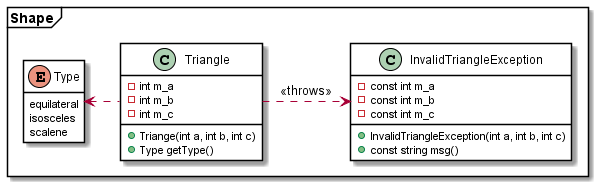
\includegraphics[scale=0.7]{figures/classdiagram.png}
    \caption{Triangle and InvalidTriangleException class UML}
    \label{fig:triangle}
\end{figure}

A main method is used to exercise the \textsc{Shape} library using user input. The main method prompts the user to input the three side lengths of the triangle, constructs a \textsc{Triangle} class object using the supplied input, and prints a string that matches the result of the getType() method.


\section{Source Code}
\begin{listing}[H]
\inputminted[breaklines,frame=single,linenos]{cpp}{code/Triangle.h}
\caption{Triangle.h}
\label{code:triangle.h}
\end{listing}


\section{Test Driver}
\begin{listing}[H]
\inputminted[breaklines,frame=single,linenos]{cpp}{code/test.cpp}
\caption{test.cpp}
\label{code:test.cpp}
\end{listing}


\section{Test Results}
\begin{figure}[H]
    \centering
    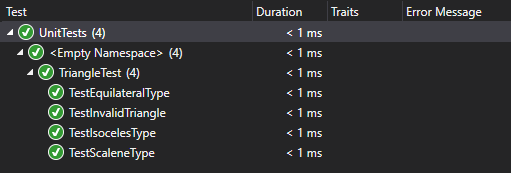
\includegraphics[scale=.8]{figures/TestResults.PNG}
    \caption{Test driver results}
    \label{fig:testresults}
\end{figure}

\end{document} 
